
This chapter describes the work done in each sprint. A sprint is one iteration of the Scrum process
(see section \ref{section:scrum} for more information about Scrum). The duration of each sprint is two weeks.
Every sprint gets assigned various tasks from the backlog and each task is given a specific point value.
This point value is an abstract estimation of the amount of work that is required to finish the task.
The point value can be also influenced by the importance of the task. If a task requires more time than
planned and is not finished by the end of the sprint, it will be assigned a 'prolonged' status and
moved to the next sprint.

\newpage

\section{Sprint 1}

Duration: 20/01 to 02/02
Points total: 92

The first sprint was dedicated to planning meetings and working hours
and studying about interested technologies. While some team members had some
experience with Arduino, none of us had any experience with Android application
development and social networks. Each member chose his own role in the project,
based on his interests. The team also did a lot of brainstorming in order
to identify possible product ideas to show the customer and produced a small
proof-of-concept application. The meeting with the customer was arranged for
the beginning of the second week.

\begin{table}[ht!]
\begin{tabular}{ | c | l | c | r | }

\hline
\textbf{ID} & \textbf{Task} & \textbf{Points} & \textbf{Status} \\
\hline

 7 & Brainstorm ideas about the product		& 18 & done \\
\hline
 8 & Search for similar products			& 14 & done \\
\hline
 9 & Proof-of-concept application			& 12 & done \\
\hline
12 & Read on OpenSocial						& 10 & done \\
\hline
13 & Read on Arduino						& 8  & done \\
\hline
11 & Read Facebook developers' pages		& 8  & done \\
\hline
10 & Choose a development process			& 6  & done \\
\hline
 6 & Meet with the customer					& 4  & done \\
\hline
10 & Read on development processes			& 4  & done \\
\hline
 2 & Plan group meetings					& 2  & done \\
\hline
 5 & Plan meetings with the customer		& 2  & done \\
\hline
 1 & Exchange contact information			& 1  & done \\
\hline
 4 & Setup mailing list						& 1  & done \\
\hline
 3 & Setup a Skype chat						& 1  & done \\
\hline
 ? & Setup a GIT repository					& 1  & done \\
\hline

\end{tabular}
\end{table}

\newpage

\begin{figure}[h!]
\centering 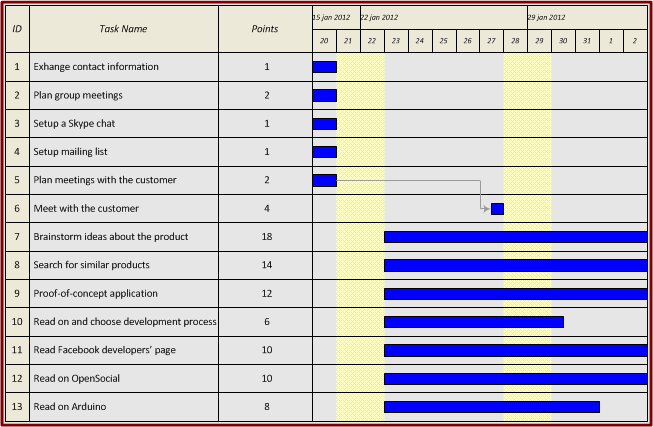
\includegraphics[scale=0.8]{img/sprints-gantt1.png}
\caption{Gantt diagram for the first sprint}
\label{fig:sprints-gantt1}
\end{figure}

\newpage


\section{Sprint 2}

Duration: 03.02 to 16.02
Points total: 99

The second iteration was focused on producing more prototypes of the product to
show the customer in order to receive the necessary feedback to identify
the product requirements and begin designing the different parts of the system,
as well as acquiring the necessary knowledge and confidence with the involved
technologies. The team also worked on the preliminary version of the report.
The customer suggested that in order to show the re-usability capabilities of
the code, two more prototypes, considerably simpler than the t-shirt prototype,
could be produced for the project.

\begin{table}[ht!]
\begin{tabular}{ | c | l | c | r | }

\hline
\textbf{ID} & \textbf{Task} & \textbf{Points} & \textbf{Status} \\
\hline

 2 & Delivery of preliminary report					& 24 & done \\
\hline
 1 & Present a working prototype (Week 1)			& 18 & done \\
\hline
 7 & Study Facebook Android SDK						& 12 & done \\
\hline
 8 & Study Android SDK								& 12 & done \\
\hline
 6 & Study Android applicationd development			& 10 & done \\
\hline
 3 & Present a working prototype (Week 2)			& 8  & done \\
\hline
 4 & Estabilish a bluetooth connection to Arduino	& 8  & done \\
\hline
 5 & Estabilish a connection to Facebook
(Facebook SDK)										& 6  & done \\
\hline
 9 & Setup ScrumDo									& 1  & done \\
\hline

\end{tabular}
\end{table}

\begin{figure}[h!]
\centering 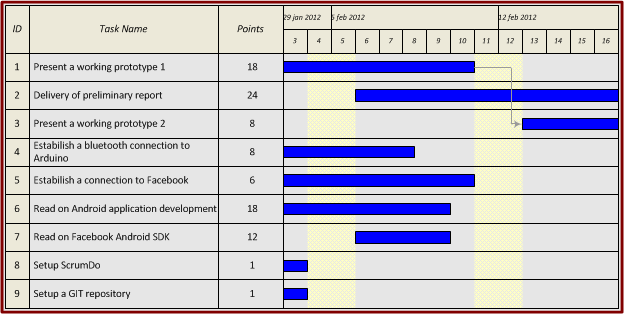
\includegraphics[scale=0.8]{img/sprints-gantt2.png}
\caption{Gantt diagram for the second sprint}
\label{fig:sprints-gantt2}
\end{figure}

\newpage

\section{Sprint 3}

Duration: 17.02 to 01.03
Points total: 108

This sprint was focused on proceeding with the design using the customer
feedback on the prototypes presented. An initial version of the Communication
library was also designed and coded. Design of the Social library also began.
During this sprint the system design started to take shape, and the parts
of the system became more definite. The team delivered a list of hardware needed
to build the various T.U.I. prototypes. The customer was happy with the team work
so far and provided very valuable feedback.

\begin{table}[ht!]
\begin{tabular}{ | c | l | c | r | }

\hline
\textbf{ID} & \textbf{Task} & \textbf{Points} & \textbf{Status} \\
\hline

 4 & Social library design (part I)					& 20 & done \\
\hline
 5 & Communication library design (part I)			& 20 & done \\
\hline
 1 & Present a working prototype (Week 1)			& 18 & done \\
\hline
 6 & Communication library coding (part I)			& 16 & done \\
\hline
 3 & Initial system design							& 14 & done \\
\hline
 7 & Read on Android IPC mechanisms					& 12 & done \\
\hline
 2 & Present a working prototype (Week 2)			& 8  & done \\
\hline

\end{tabular}
\end{table}

\begin{figure}[h!]
\centering 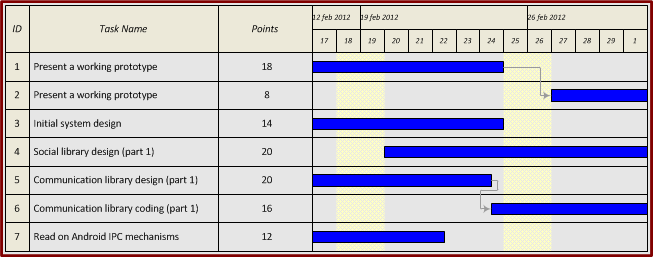
\includegraphics[scale=0.8]{img/sprints-gantt3.png}
\caption{Gantt diagram for the third sprint}
\label{fig:sprints-gantt3}
\end{figure}

\newpage


\section{Sprint 4}

Duration: 02.03 to 15.03
Points total: 112

This sprint was mainly aimed to the delivery of the mid-term report as well
as polishing of the Communication library. The system design was revised in
order to suit the customer requirements. The design of the Social library couldn't
be completed in time due to design issues. These issues were presented to the
customer who provided valuable feedback that helped solve them. The team will hopefully
receive our hardware in the next weeks, before Easter vacation. During this sprint the team
faced some issues regarding the design of the Social library and had a hard time trying
to settle for a satisfying design. The development wasn't proceeding as smoothly as planned.

\begin{table}[ht!]
\begin{tabular}{ | c | l | c | r | }

\hline
\textbf{ID} & \textbf{Task} & \textbf{Points} & \textbf{Status} \\
\hline

 1 & Work on the report				& 24 & done \\
\hline
 2 & Present a working prototype	& 18 & done \\
\hline
 3 & System design					& 18 & done \\
\hline
 7 & Comm. library coding (part II)	& 16 & done \\
\hline
 4 & Social libray design (part II)	& 14 & prolonged \\
\hline
 6 & Comm. library design (part II)	& 12 & done \\
\hline
 5 & Social library coding (part I)	& 10 & done \\
\hline

\end{tabular}
\end{table}

\begin{figure}[h!]
\centering 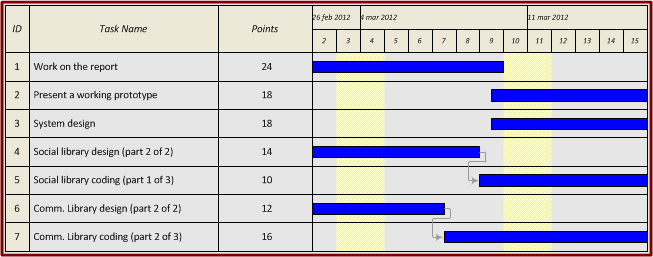
\includegraphics[scale=0.8]{img/sprints-gantt4.png}
\caption{Gantt diagram for the fourth sprint}
\label{fig:sprints-gantt4}
\end{figure}

\newpage

\section{Sprint 5}

Duration: 16.03 to 29.03
Points total: 128

During this sprint the team produced yet another prototype for the customer
and proceeded with the design and coding of the Social library.
Coding of the Communication library also continued, and an initial version
was deployed by the end of the sprint. The team also did some brainstorming
and identified the other two prototypes that were to be presented together with
the T-Shirt prototype. Some proof-of-concept applications for these
prototypes were also made. This sprint was a bit more intense than the previous
ones to cope with the fact that the next sprint would have coincided with Easter vacation.
The team still had not received the hardware needed in order to begin building the t-shirt
prototype.

\begin{table}[ht!]
\begin{tabular}{ | c | l | c | r | }

\hline
\textbf{ID} & \textbf{Task} & \textbf{Points} & \textbf{Status} \\
\hline

 2 & Social library design (part II)			& 24 & completed \\
\hline
 4 & Communication library coding (part III)	& 22 & done \\
\hline
 3 & Social library coding (part II)			& 20 & done \\
\hline
 1 & Present a working prototype				& 18 & done \\
\hline
 5 & Deploy the Comm. library					& 14 & done \\
\hline
 7 & Temperature prototype coding (part I)		& 10 & done \\
\hline
 9 & Led prototype coding (part I)				& 10 & done \\
\hline
 6 & Temperature Prototype research				& 6  & done \\
\hline
 8 & Led prototype research						& 4  & done \\
\hline


\end{tabular}
\end{table}


\begin{figure}[h!]
\centering 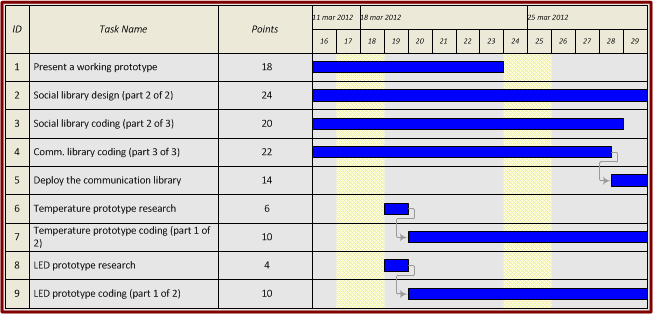
\includegraphics[scale=0.8]{img/sprints-gantt5.png}
\caption{Gantt diagram for the fifth sprint}
\label{fig:sprints-gantt5}
\end{figure}


\newpage

\section{Sprint 6}

Duration: 30.03 to 12.04
Points total: 50

As this sprint coincided with Easter vacation, little was planned for this sprint
except some early work on the report and some coding for the Social library and the second prototype.
Some team members left the city, others left the country. No meetings with the customer were arranged.
The team had a brief, sort of 'unplanned' meeting right before the vacation during which they
were told that the hardware hadn't yet been ordered.

\begin{table}[ht!]
\begin{tabular}{ | c | l | c | r | }

\hline
\textbf{ID} & \textbf{Task} & \textbf{Points} & \textbf{Status} \\
\hline

1 & Work on the report					& 18 & done \\
\hline
2 & Social library coding (part III)	& 16 & done \\
\hline
3 & Temperature prototype coding (II)	& 16 & done \\
\hline

\end{tabular}
\end{table}

\begin{figure}[h!]
\centering 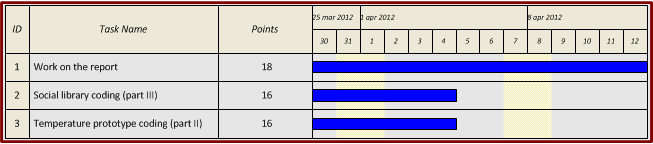
\includegraphics[scale=0.8]{img/sprints-gantt6.png}
\caption{Gantt diagram for the sixth sprint}
\label{fig:sprints-gantt6}
\end{figure}

\newpage

\section{Sprint 7}

Duration:
Points total:

Back from Easter vacation! Roughly one week after the group
was back from Easter vacation, the necessary hardware components needed for the product
had arrived. Mr. Babak, our customer, kindly bought for us a jacket that was to be used
for the final product. The Social library was finished and deployed.
Coding for the final T-shirt application began. The team started integrating
and testing the various parts of the system together; the various hardware devices were
hooked up with the Lilypad board and then tested, along with the Communication library,
using a mockup application.

During this sprint the final product changed sightly from a T-shirt to a jacket.
The Lilypad board probably wasn't the best choice for a jacket product, in fact,
since the Arduino board could be hidden in a pocket, the team could have used a smaller
and more 'soldering-friendly' Arduino board, maybe with power connector.

\begin{table}[ht!]
\begin{tabular}{ | c | l | c | r | }

\hline
\textbf{ID} & \textbf{Task} & \textbf{Points} & \textbf{Status} \\
\hline


1 & Building the prototype	(part I)	& 16 & done \\
\hline
2 & Integration testing		(part I)	& 20 & done \\
\hline
2 & System testing			(part I)	& 12 & done \\
\hline
3 & Comm. library testing	(part I)	& 10 & done \\
\hline
4 & Social library testing	(part I)	& 6  & done \\
\hline
5 & T-Shirt application coding (part I)	& 20 & done \\
\hline


\end{tabular}
\end{table}



\newpage

\section{Final sprint}

Duration:
Points total:

\begin{figure}[h!]
\centering 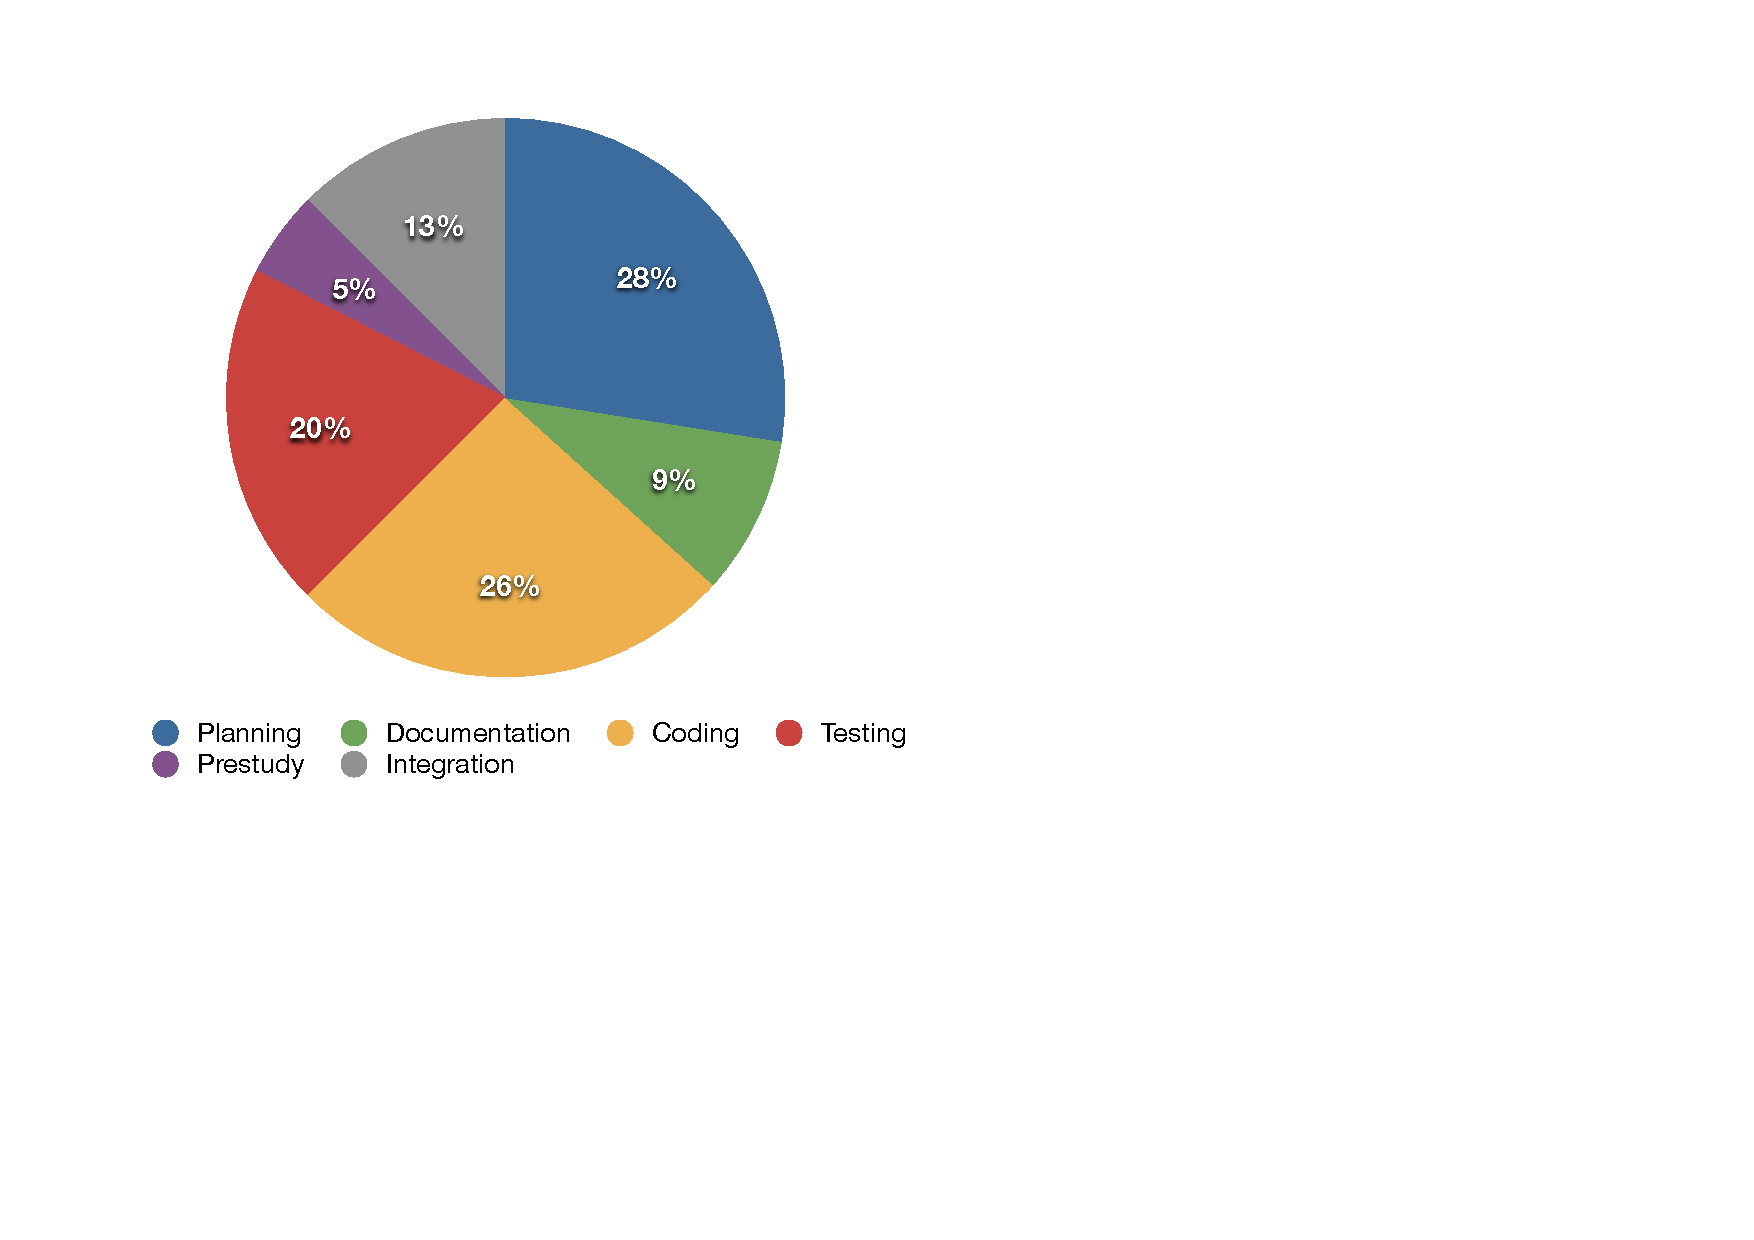
\includegraphics[scale=0.8]{img/pie_chart.pdf}
\caption{Story points breakdown}
\label{fig:sprints-points}
\end{figure}
